\section{Any-Scale Deep Network (ASDN\cite{ASDN})}

\textbf{ASDN} and \textit{Meta-SR\cite{MetaSR}}[\Cref{metasr}] are few among SR networks whose objective is to achieve SR images using decimal scales.

In order to do so \textit{Meta-SR} used a \textit{meta-upscaling module} which learns the weights used for convolving features extracted by a LR image given the scale; therefore \textit{Meta-SR}  is able to predict the SR image only for scales used for training.

For overcoming this and the impossibility to train a network for all possible decimal scales, \textit{ASDN} eases the task using a \textbf{Laplacian Frequency Representation}: exploiting the Laplacian Framework with decimal scales (seen in \Cref{lapsrn}) the SR image is reconstructed interpolating two nearest neighbors of the decimal scale in the laplacian pyramid.

\subsection{Laplacian Frequency Representation}
\begin{figure}
    \centering
    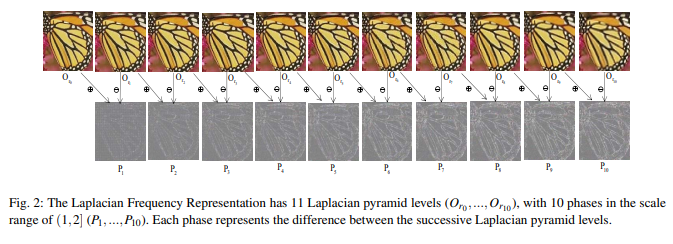
\includegraphics[width=\textwidth, keepaspectratio]{asdn-laplacian-pyramid.png}
    \caption{Laplacian Frequency Representation using decimal scales}\label{asdn:lfr}
\end{figure}

Each level learns the high frequency image at the specific scale which is defined as:
$$
r_l = \frac{l}{L-1} + 1
$$
then given any decimal scale \textbf{r} the nearest neighbor is chosen with:
$$
i = \left\lceil (L-1) \ast (r-1) \right\rceil
$$
and the weights used for interpolating are:
$$
w_r  = (L-1) \ast (r_i - r)
$$
therefore the \textbf{SR image} is:
$$
O_r = O_{r_i} + w_r \ast P_i
$$
where $P_i = O_{r_{i-1}} - O_{r_i}$  

The pyramid is named \textit{Laplacian Frequency Representation} (\textit{LFR}) because at each level a phase is computed which represents the high frequency information of the input image as if we are applying a laplacian operator, indeed looking at \Cref{asdn:lfr} what we have is a sort of edge detector.

\subsection{Recursive deployment}
In order to avoid to train the network for all possible decimal scales  the \textit{Laplacian Frequency Representation} is fixed to a range therefore in order to be able to upscale decimal scales greater thant the greatest scale in the pyramid the network is deployed recursively.
In general a large scale $R$ can be defined as $R = r^N$ where $N$ is the number of recursions.

The best scales range is found to be $\left(1,2 \right]$ therefore the network should be deployed $N-1$ times with $r=2$ and once with $r=\frac{R}{2^{N-1}}$ where $N=\left\lceil\log_2 R \right\rceil$

\subsection{Architecture}
\begin{figure}
    \centering
    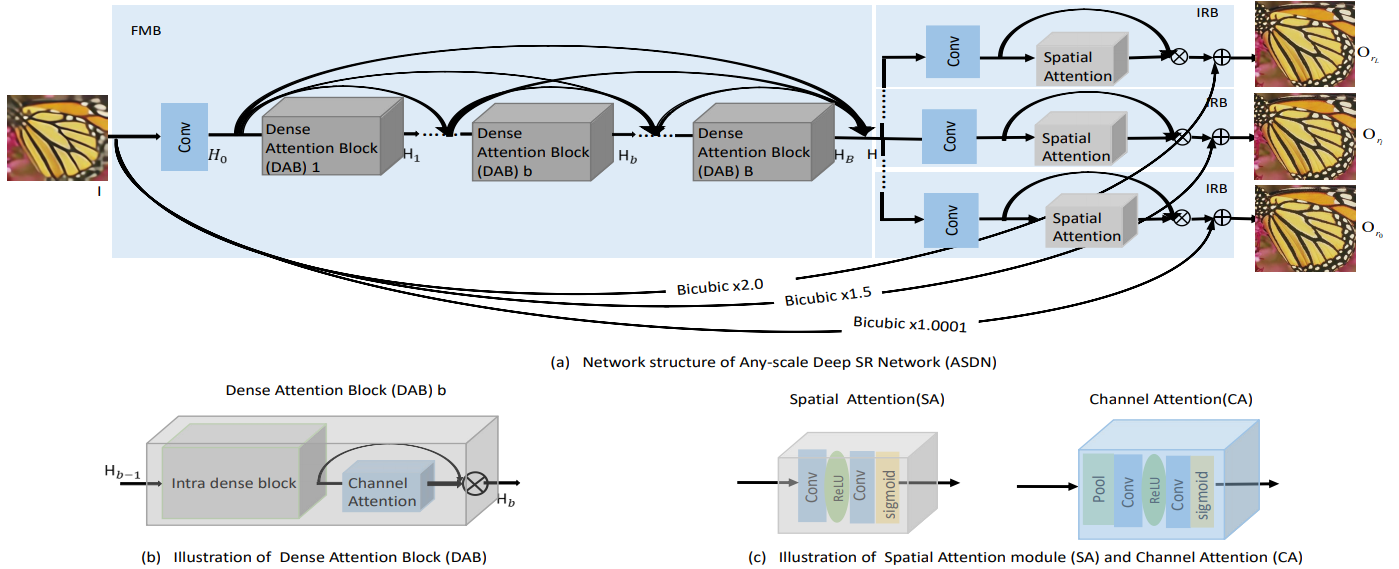
\includegraphics[width=\textwidth, keepaspectratio]{asdn-architecture.png}
    \caption{ASDN architecture}\label{asdn:model}
\end{figure}

Looking at [\Cref{asdn:model}], ASDN has:
\begin{itemize}
    \item a shallow features extractor
    \item a deeper features extractor, \textbf{Feature Mapping Branch} (\textit{FMB})
    \item at each level in the \textit{LFR} the features are reconstructed using the \textbf{Image Reconstruction Branch} (\textit{IRB})
    \item the \textit{FMB} is shared among all \textit{IRBs}
\end{itemize}

The \textit{ASDN} is the aggregator of all previous studies:
\begin{itemize}
    \item the \textbf{bi-dense connections} allow to reuse all features within the network, maintain long-term information and ease the training avoiding vanishing/exploding gradient (seen in \Cref{dbdn})
    \item the IDBs taken directly from \Cref{dbdn} allow to maintain short-term information focusing the training on most important features thanks ot the \textbf{channel attention}(as seen in \Cref{rcan} and \Cref{csfm})
    \item the IRB project the features in the image space using a 1x1 convolution with $C=3$ (or 1 in case of gray-scale images) and then the reconstruction is focused on particular region where high-frequency information are laying due to the \textbf{spatial attention} mechanism (as seen in \Cref{csfm})
\end{itemize}

\subsection{FSDN}
\textit{Fixed-scale deep network} (\textbf{FSDN}) is a network similar to ASDN, with the only exception of a transposed convolution at the beginning of each IRB, which is fine tuned to a specific scale.

\subsection{Results}

\subsubsection{Efficiency of the Laplacian Frequency Representation and density study.}
Looking at [\Cref{asdn:lfrstudies}] the Laplacian Frequency Representation (network trained using 11 IRBs: EDSR-Conv, RDN-Conv, ASDN) has the same performances of networks trained using pre-upsampling method (EDSR-100, RDN-100, ADSN-100 on 100 scales between 1 and 2).

We can see that the denser the pyramid the better but at some point it saturate and no benefit are achieved (ASDN-\textbf{x} where $x$ is the number of phases in the LFR so $L=x+1$.)

\begin{figure}[H]
    \centering
    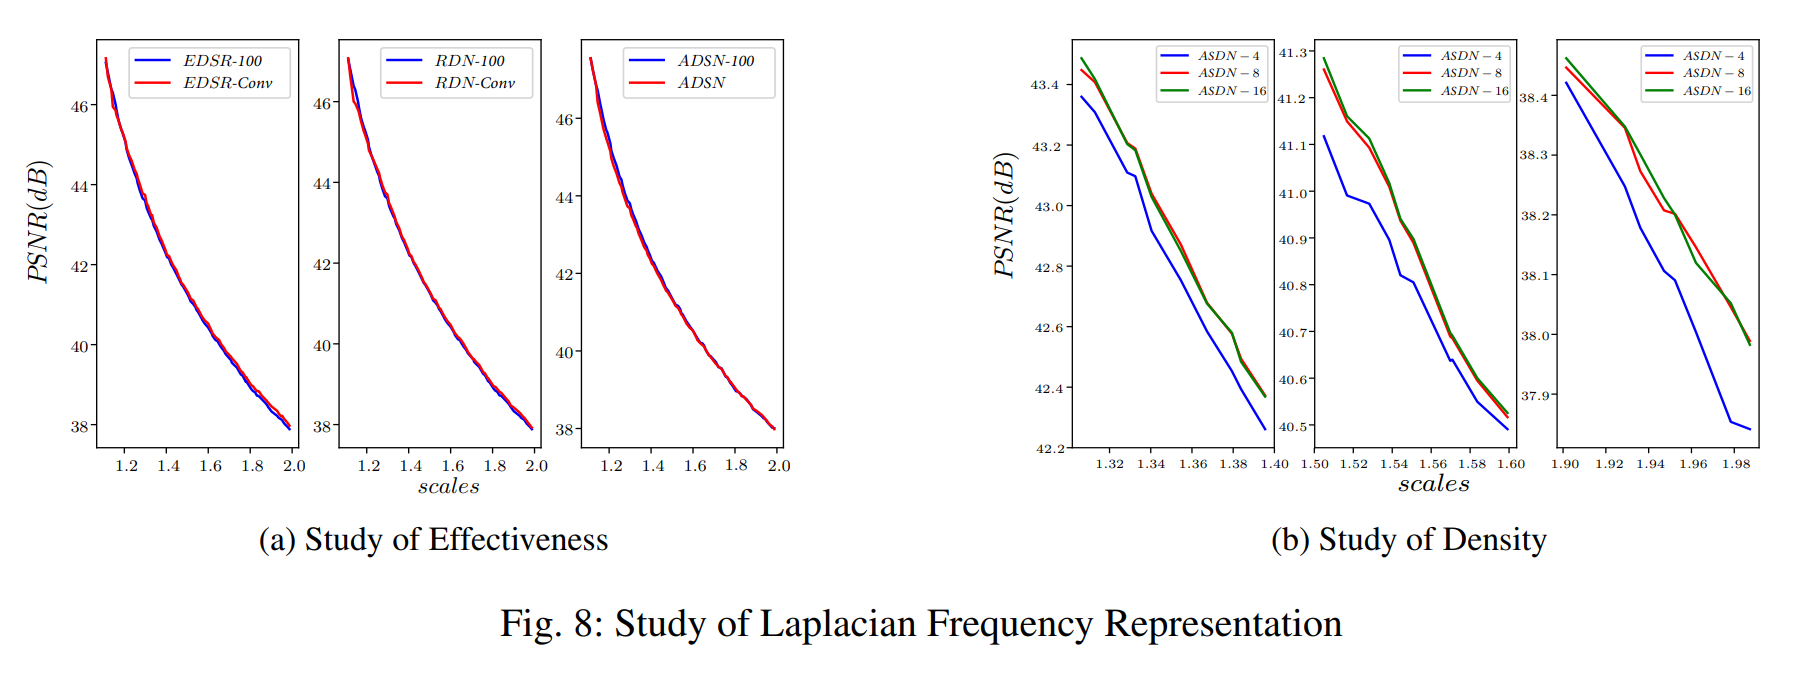
\includegraphics[width=\textwidth, keepaspectratio]{asdn-study-lfr.png}
    \caption{Effectiveness and density of LFR.}\label{asdn:lfrstudies}
\end{figure}

\subsubsection{Efficiency of the recursive deployment and optimal N and r}
The direct deployment uses networks trained with images upscaled directly to x2,x3,x4 instead recursive deployment uses networks trained twice using $x\sqrt{2}$, $x\sqrt{3}$,$x\sqrt{4}$.

From [\Cref{asdn:rds}] we can see that the difference in performance is noticeable with lower scales and decrease  with it and using the greatest scale at the beginning lead to better performance.

\begin{figure}[H]
    \begin{subfigure}{\textwidth}
        \centering
        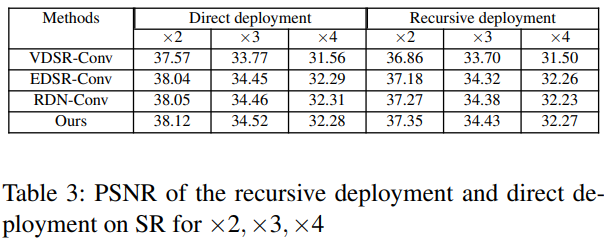
\includegraphics[width=\textwidth, keepaspectratio]{asdn-study-rd.png}
        \caption{Study of the effectiveness of the recursive deployment.}        
    \end{subfigure}
    \begin{subfigure}{\textwidth}
        \centering
        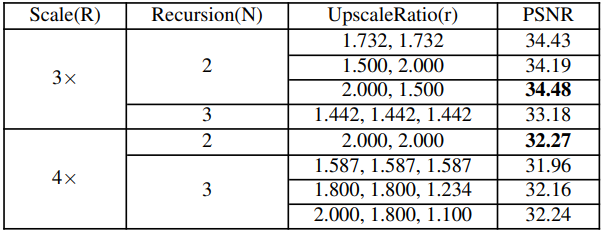
\includegraphics[width=\textwidth, keepaspectratio]{asdn-study-n-rd.png}
        \caption{Optimal N and r for the recursive deployment.}
    \end{subfigure}
    \caption{Recursive deployment studies.}\label{asdn:rds}
\end{figure}


\subsubsection{Ablation studies and performance versus parameters}
Every component inside ADSN is important for achieving better performance as shown in \Cref{asdn:ablation-studies}.

The network is able to achieve state-of-the-art performance with a small amount of parameters (22M).

\begin{figure}[H]
    \begin{subfigure}{\textwidth}
        \centering
        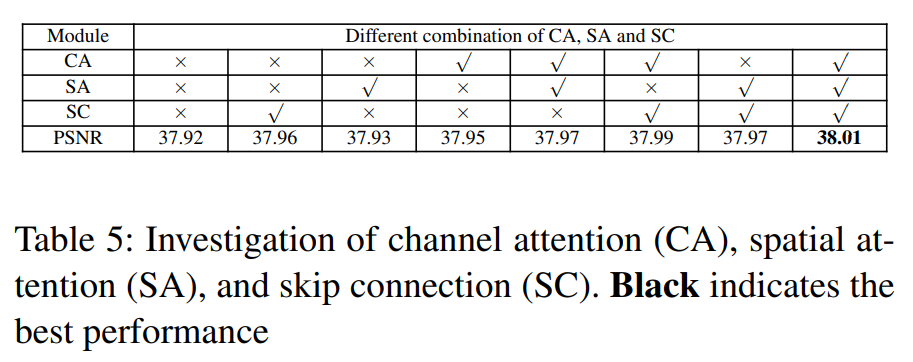
\includegraphics[width=\textwidth, keepaspectratio]{asdn-ablation-study.png}
        \caption{Ablation studies on channel attention (CA), spatial attention (SA) and global skip connection (SC).}\label{asdn:ablation-studies}
    \end{subfigure}
    \begin{subfigure}{\textwidth}
        \centering
        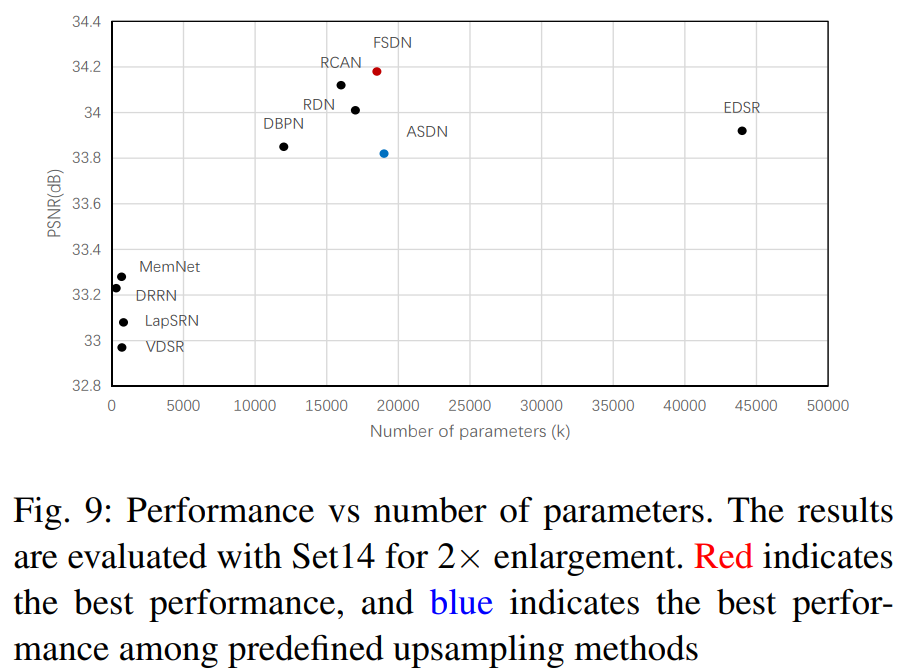
\includegraphics[width=\textwidth, keepaspectratio]{asdn-psnr-n_params.png}
        \caption{PSNR versus number of parameters.}
    \end{subfigure}    
\end{figure}

\subsubsection{Quantitative and qualitative results}

\paragraph{Fixed scales}
Overall ASDN performs better than any predefined upsampling method and FSDN has the best performance (this highlight the fact that having learnable upscaling method allow to achieve better performance).

Sometimes ASDN performs worse because some network are trained specifically for a particular scales with the particular dataset or it is worse than RCAN because has many channel attention modules that allow to improve the reconstruction.
\begin{figure}[H]
    \centering
    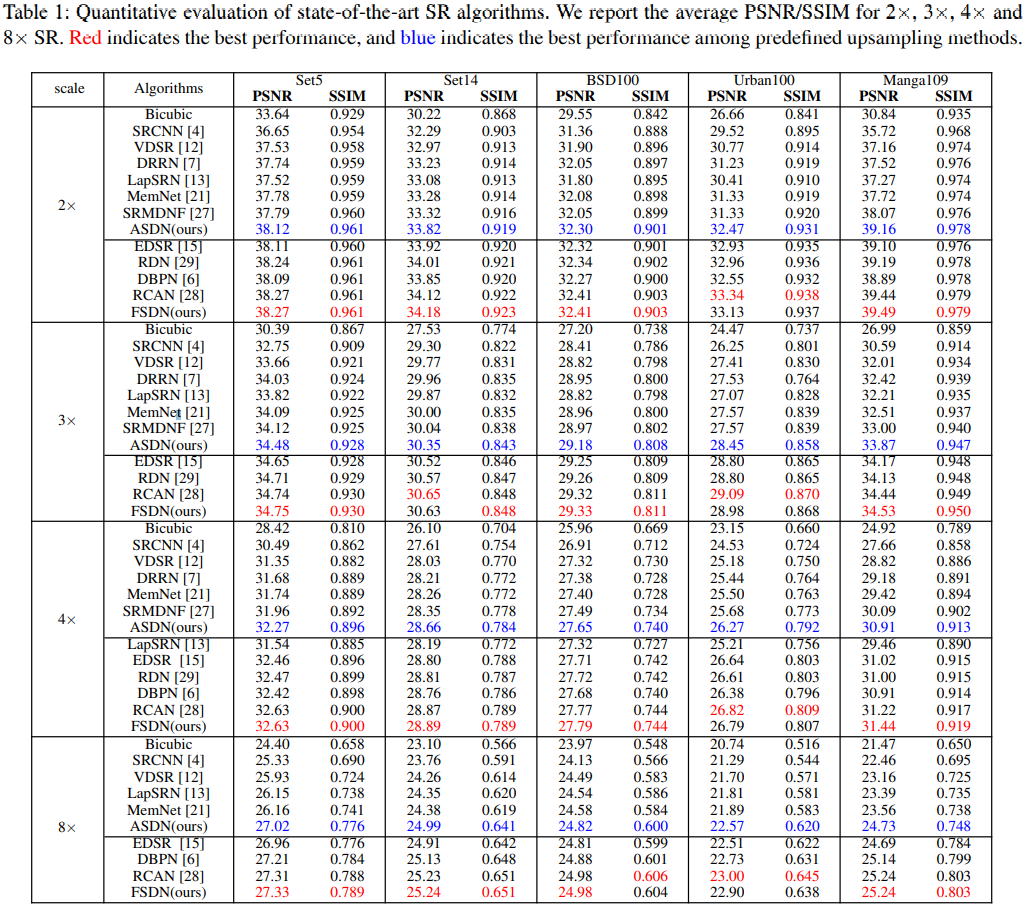
\includegraphics[width=\textwidth, keepaspectratio]{asdn-table1.png}
    \caption{Comparison of quantitative results using fixed scales.}
\end{figure}

\paragraph{Any-scale}
ASDN performs better than state-of-the-art for upsampling images using decimal scales used or not for training.
\begin{figure}[H]
    \begin{subfigure}{\textwidth}
        \centering
        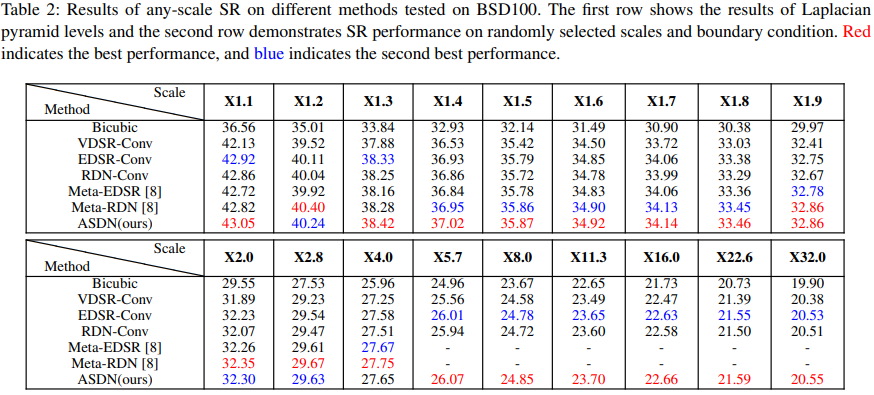
\includegraphics[width=\textwidth, keepaspectratio]{asdn-table2.png}
        \caption{Comparison of quantitative results using decimal scales.}
    \end{subfigure}
    \begin{subfigure}{\textwidth}
        \centering
        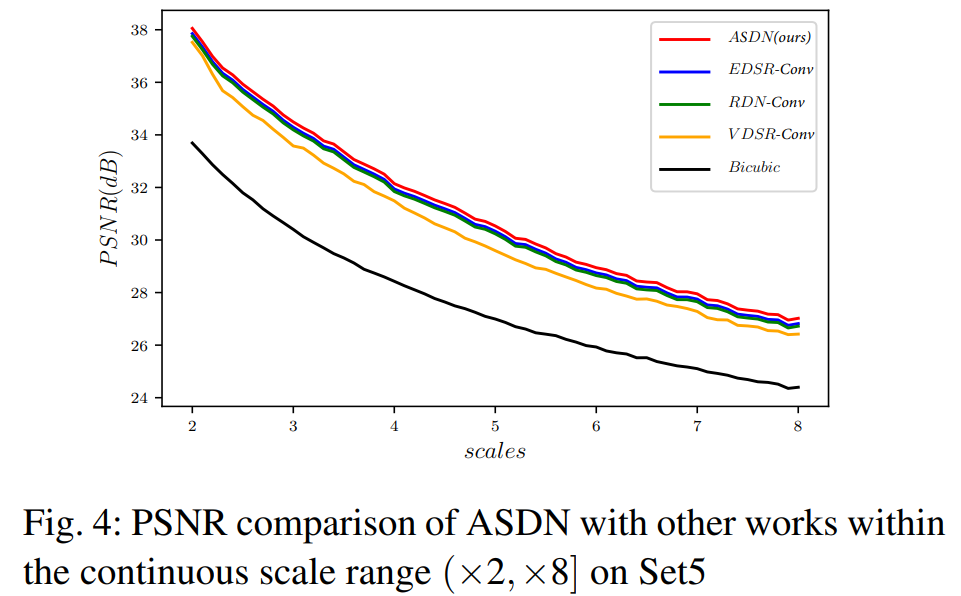
\includegraphics[width=\textwidth, keepaspectratio]{asdn-fig4.png}
        \caption{Comparison of quantitative results using decimal scales between 2 and 8.}
    \end{subfigure}
\end{figure}

\paragraph{Qualitative results}
The visual quality of ASDN is similar to state-of-the-art and FSDN outperforms state-of-the-art networks.

\begin{figure}
    \centering
    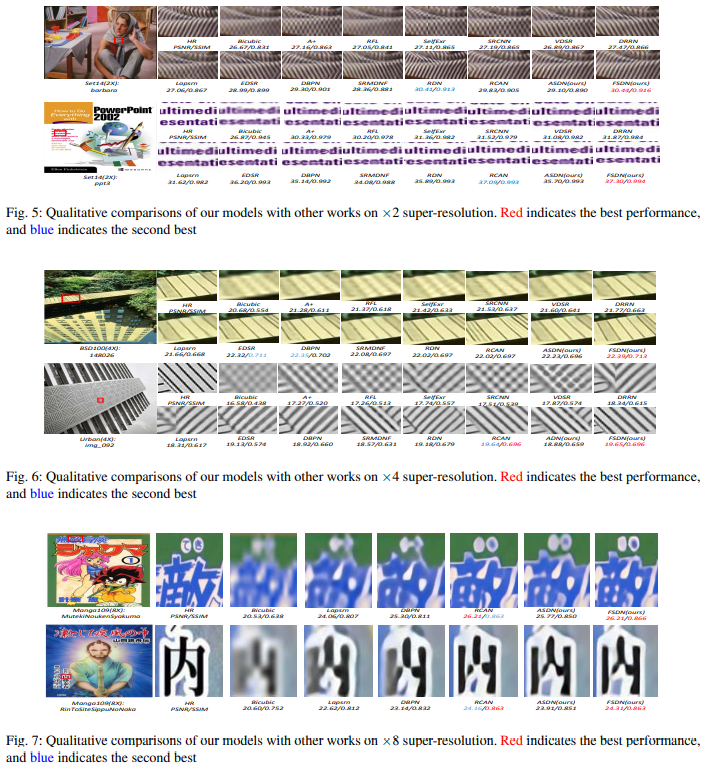
\includegraphics[width=\textwidth, keepaspectratio]{asdn-qulitative-results.png}
    \caption{Qualitative results of ASDN and FSDN on different datasets.}
\end{figure}

